\section{Formální konceptuální analýza (FCA)}
Metoda analýzy tabulkových dat (objektů a jejich vlastností), umožňuje jiný pohled na data (využívá se např. u data miningu). \textbf{Vstupem} pro FCA jsou \textbf{tabulková data}, která jsou uspořádána následovně: \textbf{objekty} (řádky) a \textbf{atributy} (sloupce). Tyto tabulková data vytváří tzv. \textbf{kontexty}.

\begin{table}[H]
    \centering
    \begin{tabular}{l|l|l}
                        & \textbf{červené} & \textbf{bílé} \\
        \hhline
        \textbf{jablko} & $\times$         &               \\
        \textbf{zelí}   & $\times$         & $\times$
    \end{tabular}
\end{table}

\section{Formální Kontext}
Formální kontext $K$ obsahuje objekty z množiny $O$ a atributy z množiny $A$. Vztahy mezi objekty a atributy jsou charakterizovány binární relací $ R $. Obecně se pro popis kontextu používá výraz:
\begin{equation}
    K = (O, A, I).
\end{equation}
Takto vymezený formální kontext je dobře zobrazitelný tabulkou, ve které jsou \textbf{řádky} obsazeny \textbf{objekty}, \textbf{sloupce} \textbf{atributy} a incidenční data ($I \subseteq O \times A$) vyjadřují relaci $ R $ ($I$ je relace incidence).

\subsection{Galoisovy konexe}
Umožňují přecházet z množiny objektů na jejich společné atributy ($\uparrow$ \textbf{intent}) a naopak ($\downarrow$ \textbf{extent}).

\begin{itemize}
    \item \textbf{Intent} $\uparrow$ -- $2^X \rightarrow 2^Y; A \subseteq X; A^\uparrow = \{y \in Y; \forall x \in A (x, y) \in I\}$ [\textit{z objektu na atributy}].
    \item \textbf{Extent} $\downarrow$ -- $2^Y \rightarrow 2^Y; B \subseteq Y; B^\downarrow = \{x \in X; \forall y \in B (x, y) \in I\}$ [\textit{z atributů na objekt}].
\end{itemize}

\subsection*{Příklad}
$A_1 = \{\textrm{jablka, zelí}\}, A_1^\uparrow = \{\textrm{červené}\}$ \quad $A_2 = \{\textrm{zelí}\}, A_2^\uparrow = \{\textrm{červené, bílé}\}$\\
$B_1 = \{\textrm{\rm červené, bílé}\}, B_1^\downarrow = \{\textrm{zelí}\}$ \quad $B_2 = \{\textrm{červené}\}, B_2^\downarrow = \{\textrm{zelí, jablko}\}$

\section{Formální koncept}
Formální koncept je dvojice $(A, B)$, kde $A$ je množina objektů, a $B$ je množina atributů, které jsou \textbf{společné pro všechny objekty} z množiny $A$. Koncept $(A, B)$ je tedy dán jako: $(A, B) \Leftrightarrow A = B^\downarrow \land B = A^\uparrow$, kde $A \subseteq X$, $B \subseteq Y$, kde $X$ a $Y$ jsou objekty a atributy výše uvedené tabulky.

\subsection{Uzávěrový operátor $\uparrow \downarrow$}
Jak již znační $A^{\uparrow \downarrow} = C(A)$ vypovídá, k určení uzávěru atributů množiny $A$ se nejprve provede \textbf{intent} a poté \textbf{extent}. Uzávěr má tyto vlastnosti:
\begin{enumerate}
    \item \textbf{Idempotence} -- $C(C(A)) = C(A)$.
    \item \textbf{Extensionalita} -- $A \subseteq C(A)$.
    \item \textbf{Monotonie} -- $A_1 \subseteq A_2 \Rightarrow C(A_1) \subseteq C(A_2)$.
\end{enumerate}

\section{Konceptuální svazy}
\textbf{Uspořádaná množina konceptů} tvoří tzv. konceptuální svaz. Ten lze graficky znázornit \textbf{Hasseovým diagramem} -- každý vrchol grafu reprezentuje \textbf{jeden koncept}. Koncepty $ K_i $ a $ K_j $ jsou v grafu spojeny, pokud $ K_i \leq K_j$, přičemž $K_j$ je umístěn výše než $K_i$ a neexistuje takové $K_k$, že $ K_i \leq K_k \leq K_j$.

\subsection{Návod k vytvoření konceptuálního svazu}
\begin{enumerate}
    \item Vytvořím a postupně si zapíšu množinu všech extentů na jednotlivých atributech (v grafu zapisuji \textbf{zdola nahoru}).
    \item Vytvořím jedinečné průniky extentů.
    \item Nesmím zapomenout na zahrnutí průniku s prázdnou množinou = $\emptyset$.
    \item Přidám extent zahrnující všechny objekty.
    \item Pro odpovídající extenty vytvořím intenty (v grafu zapisuji \textbf{shora dolů}).
\end{enumerate}

\subsection*{Příklad}
\begin{table}[H]
    \centering
    \begin{tabular}{l|l|l|l|l}
                         & \textbf{2 nohy} & \textbf{4 nohy} & \textbf{mléko} & \textbf{vlna} \\\hhline
        \textbf{pes}     &                 & $\times$        &                &               \\
        \textbf{ovce}    &                 & $\times$        & $\times$       & $\times$      \\
        \textbf{koza}    &                 & $\times$        & $\times$       &               \\
        \textbf{slepice} & $\times$        &                 &                &               \\
    \end{tabular}
\end{table}

\begin{minipage}[t]{0.5\textwidth}
    $e_7 = \{$pes, ovce, koza, slepice$\}$\\
    $e_2 = \{\textrm{4 nohy}\}^\downarrow = \{\textrm{pes, ovce, koza}\}$\\
    $e_3 = \{\textrm{mléko}\}^\downarrow = \{\textrm{ovce, koza}\}$\\
    $e_1 = \{\textrm{2 nohy}\}^\downarrow = \{\textrm{slepice}\}$\\
    $e_4 = \{\textrm{vlna}\}^\downarrow = \{\textrm{ovce}\}$\\
    $e_5 = e_2 \cap e_3 = \{\textrm{ovce, koza}\}$\\
    $e_6 = \emptyset$
\end{minipage}
\begin{minipage}[t]{0.5\textwidth}
    $i_7 = e_7^\uparrow = \emptyset$\\
    $i_2 = e_2^\uparrow = \{\textrm{4 nohy}\}$\\
    $i_3 = e_3^\uparrow = \{\textrm{4 nohy, mléko}\}$\\
    $i_1 = e_1^\uparrow = \{\textrm{2 nohy}\}$\\
    $i_4 = e_4^\uparrow = \{\textrm{4 nohy, mléko, vlna}\}$\\
    $i_5 = e_5^\uparrow = \{\textrm{4 nohy, mléko}\}$\\
    $i_6 = e_6^\uparrow = \{\textrm{2 nohy, 4 nohy, mléko, vlna}\}$\\
\end{minipage}

\begin{center}
    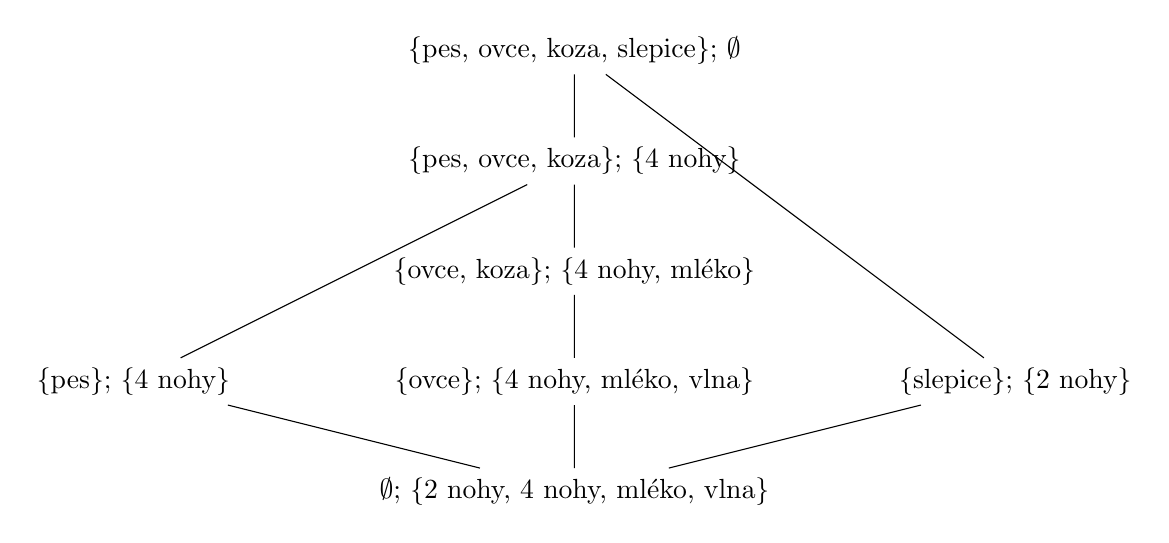
\begin{tikzpicture}[scale=.7]
        \node (e6) at (0,-4) {$\emptyset$; \{2 nohy, 4 nohy, mléko, vlna\}};
        \node (e5) at (-8,-2) {\{pes\}; \{4 nohy\}};
        \node (e4) at (0,-2) {\{ovce\}; \{4 nohy, mléko, vlna\}};
        \node (e1) at (8,-2) {\{slepice\}; \{2 nohy\}};
        \node (e3) at (0,0) {\{ovce, koza\}; \{4 nohy, mléko\}};
        \node (e2) at (0,2) {\{pes, ovce, koza\}; \{4 nohy\}};
        \node (e7) at (0,4) {\{pes, ovce, koza, slepice\}; $\emptyset$};
        \draw (e6) -- (e5) -- (e2) -- (e7) -- (e1) -- (e6) -- (e4) -- (e3) -- (e2);
    \end{tikzpicture}
\end{center}

\section{Svazy (pro doplnění)}
Svaz je algebra $(L, \cap, \cup)$ s dvěma základními binárními operacemi $x\cap{}y$ \textbf{spojení (suprémum)} (sup(x, y)) a $x\cup{}y$ \textbf{průsek (infimum)} (inf(x, y)), které mají následující vlastnosti:
\begin{enumerate}
    \item \textbf{Univerzalita (jednoznačnost)} -- $\forall x,y \,\exists z \,\,\, x \cap y = z\quad|\quad\forall x,y \exists\, z \,\,\, x \cup y = z$.
    \item \textbf{Asociativita} -- $x \cap (y \cap z) = (x \cap y) \cap z \quad|\quad x \cup (y \cup z) = (x \cup y) \cup z$.
    \item \textbf{Komutativita} -- $x \cap y = y \cap x \quad|\quad x \cup y = y \cup x$.
    \item \textbf{Absorbce} -- $x \cap (x \cup y) = x \quad|\quad x \cup (x \cap y) = x $.
\end{enumerate}

\subsection{Typy svazů}
\begin{enumerate}
    \item \textbf{Distributivní} -- platí zde axiomy distributivity a neobsahuje ani \textbf{diamant} ani \textbf{pentagon}: $x \cup (y \cap z) = (x \cup y) \cap (x \cup z) \quad|\quad x \cap (y \cup z) = (x \cap y) \cup (x \cap z) $.

          \begin{figure}[H]
              \centering
              \includegraphics[width=.4\textwidth]{assets/pentagon_diamant}
          \end{figure}
    \item \textbf{Modulární} -- slabší reprezentace distributivity, \textbf{nesmí} obsahovat \textbf{pentagon}, $a \geq c: a \land (b \lor c) = (a \land b) \lor c$.
    \item \textbf{Komplementární} -- platí zde, že pro každý prvek $ x $ existuje komplement $x' $, kdy: $x \cap x' = $ [svazová 0] a $x \cup x' = $ [svazová 1]
    \item \textbf{Booleovský svaz} -- komplementární $\land$ distributivní
\end{enumerate}

\subsection{Vlastnosti svazů}
Pro každé dva prvky v množině existuje \textbf{sup} a \textbf{inf}. \textbf{Úplný svaz} -- nastane tehdy, zda pro \textbf{libovolné neprázdné podmnožiny existuje} sup a inf. U svazů můžeme dále získat tyto vlastnosti:
\begin{itemize}
    \item \textbf{Minimum a maximum} -- žádný není menší/větší než $a$ (vrchol diagramu).
    \item \textbf{Nejmenší a největší} -- \textbf{pouze jeden} nejmenší/největší prvek, pokud je jich více, \textbf{neexistuje} největší/nejmenší prvek.
    \item \textbf{Dolní (L(A)) a horní (U(A)) závora} -- všechny prvky jsou $\leq/\geq$ než A,
    \item \textbf{Infimum} -- nejmenší prvek dolní závory.
    \item \textbf{Supremum} -- nejmenší prvek horní závory.
\end{itemize}